\documentclass{article}
\usepackage{biblatex}
\addbibresource{literature.bib}

\usepackage{graphicx}
\usepackage[english]{babel}
\usepackage{caption}
\usepackage{csquotes}
\usepackage{xcolor}
\usepackage{subcaption}
\usepackage{authblk}
\usepackage{colortbl}
\usepackage{mathtools}
\usepackage{placeins}
\usepackage{graphicx}%
\usepackage{multirow}%
\usepackage{textcomp}%
\usepackage{booktabs}%
\usepackage{listings}%
\usepackage{siunitx}
\usepackage[colorinlistoftodos]{todonotes}
\usepackage{hyperref}
\usepackage{soul}
\usepackage{makecell}

%\setlength{\textwidth}{6.5in}
\usepackage[a4paper, total={5in, 7in}]{geometry}

\graphicspath{figures/}

\title{Advancing Reinforcement Learning Control: Continuous Scheme and Curriculum Learning for Mechanical Systems}

\author[1,2]{Oleg Rogov} 
\author[3]{Peter Manzl}
\author[3]{Johannes Gerstmayr}
\author[2]{Grzegorz Orzechowski}
\affil[1]{Savonia University of Applied Sciences}
\affil[2]{Lappeenranta-Lahti University of Technology LUT}
\affil[3]{University of Innsbruck}

% \date{January 2024}

\begin{document}

\maketitle

\listoftodos

\section{Introduction}

Multibody System Dynamics (MSD) is a field of study that concentrates on modeling, simulating, and analyzing the dynamics of systems composed of interconnected rigid and flexible bodies. It is a fundamental approach to understanding and predicting the dynamic behavior of complex mechanical systems through sophisticated mathematical models and computational algorithms. The essence of MSD lies in its capacity to accurately describe the motion, forces, and interactions among the components of a system and with the environment, considering both translational and rotational movements and the constraints that govern these movements~\cite{shabana2013dynMSD}. MSD is applicable across various engineering fields, from aerospace and automotive to biomechanics and robotics. This versatility underscores its capability to address the specific dynamics of different systems, enhancing its utility in diverse technological and scientific domains. Also, by accurately predicting system behavior, MSD supports the iterative design and optimization of mechanical systems. Engineers can use MSD to test and refine designs virtually, reducing the need for physical prototypes and accelerating the development process. One important characteristic of MSD is that the detailed models developed using this method make it an excellent foundation for implementing learning-based or model-based control strategies. These strategies, such as Reinforcement Learning (RL)~\cite{sutton_reinforcement_2018} and Model Predictive Control~\cite{schwenzer2021mpc}, can dynamically adapt to the system's behavior, leading to optimized performance even in complex and changing environments.

Reinforcement Learning, a primary control method used in our research, is a branch of Machine Learning (ML) where an agent learns to make decisions by taking actions in an environment to maximize the cumulative reward under acting according to a certain policy~\cite{sutton_reinforcement_2018}. In RL, rewards may not be immediate. An agent may need to perform a series of actions before receiving a reward, creating a delay between the initial action and the eventual reward. The learning process involves exploring various actions and states (exploration) and exploiting the knowledge gained to make better decisions (exploitation). The exploration and exploitation trade-off is one of the crucial concepts in reinforcement learning (RL), which emphasizes the need for a balance that results in efficient agent training. Achieving this balance is essential for the agent to learn effectively and optimize its performance over time. RL can be divided into two main types: model-free methods and model-based methods. The main difference between them is that in model-free methods the agent learns directly from interactions with the environment without trying to understand its dynamics, while in model-based methods the agent learns a model of the environment's dynamics and uses this model to plan and make decisions. Model-free methods are generally simpler and more robust in highly dynamic and complex environments, though they require more interactions for an agent to learn effectively. 
Additionally, RL can be further categorized into traditional Reinforcement Learning (RL) and Deep Reinforcement Learning (DRL). Traditional RL focuses on methods where the agent typically operates with simpler, lower-dimensional state spaces. These methods often rely on tabular representations or linear function approximations. DRL, however, specifically integrates deep neural networks to approximate value functions or policies, so that it can effectively handle high-dimensional state spaces and complex environments. This capability allows DRL to be applied to tasks such as playing video games, robotic control, and autonomous driving~\cite{roveda2020mbrl, mnih2013dqn, zhu2022inverted}. Examples of DRL methods are Advantage-Actor Critic (A2C), Proximal Policy Optimization (PPO) and Deep Q-Network (DQN). A2C is an advanced version of the actor-critic method that uses both policy (actor) and value (critic) functions, with the actor updating the policy based on feedback from the critic, enhancing stability and performance~\cite{mnih2016a2c}. PPO is a popular policy gradient method known for its robustness and simplicity, utilizing a clipped objective function to ensure stable learning~\cite{schulman2017ppo}. DQN combines Q-learning~\cite{sutton_reinforcement_2018} with deep neural networks to handle high-dimensional state spaces, approximating the Q-value function, which represents an expected cumulative reward an agent can achieve by taking a specific action in a given state and following the optimal policy, enabling it to learn effective policies in complex environments~\cite{mnih2013dqn}. 
In Reinforcement Learning, actions (control inputs) can be either discrete or continuous. Discrete actions are suitable for tasks where the set of possible actions is limited and distinct, such as choosing between different predefined options. Continuous actions, on the other hand, are used in scenarios where actions can take any value within a range, such as adjusting the speed of a car or the angle of a robotic arm. 
% RL is inspired by behavioral psychology and is gaining popularity in robotics, game playing, and optimization problems~\cite{roveda2020mbrl, mnih2013dqn, zhu2022inverted}.

The application of RL techniques in the context of MSD is still an emerging field, with limited research available. Current studies have primarily focused on traditional control methods, leaving significant potential for further exploration and development of RL-based approaches to enhance the adaptability and efficiency of MSD models. A noticeable study in this area is done by Kurinov et al.~\cite{kurinov2020autoexcavator}. Researchers have developed an autonomous excavator system utilizing RL as a control base integrated with MSD (detailed simulation with hydraulics and sensors). This study was focused on enabling the excavator to perform various tasks autonomously, including excavation and loading. The effectiveness of their approach was demonstrated in achieving autonomous operation with minimal collisions, showcasing the potential for automation in heavy machinery within the construction and mining industries.  
Additionally, Egli et al.~\cite{egli2022soil} explored the application of reinforcement learning (RL) for adaptive control in hydraulic excavators, aiming to enhance the automation of excavation tasks. Their study introduced a controller capable of adjusting to varying soil properties within a single excavation cycle. Utilizing an RL-based approach, they trained a control policy in simulation, integrating proprioceptive measurements to infer soil characteristics. This method demonstrated significant improvements in adaptability and efficiency compared to traditional excavation techniques. Notably, their controller could operate without explicit soil parameter inputs, relying instead on measurements from hydraulic pressure and kinematic sensors. The experiments conducted on a 12-ton excavator confirmed the controller's ability to maintain high performance across diverse soil conditions, emphasizing the feasibility of RL in real-world excavation scenarios.
Furthermore, Osa and Aizawa~\cite{osa2022deep} investigated deep reinforcement learning with adversarial training for automated excavation. They proposed a novel regularization method that employs virtual adversarial samples to mitigate the overestimation of Q-values in a Q-learning algorithm. Their approach, which integrates depth images for excavation planning, demonstrated superior sample efficiency and robustness in policy learning compared to traditional actor-critic methods~\cite{sutton_reinforcement_2018}. This research highlights the importance of incorporating visual information and advanced regularization techniques to enhance the reliability and effectiveness of RL-based systems.

While RL has shown considerable promise as a control method for complex dynamic systems, it is not without its limitations. One of the primary challenges of RL is its high demand for extensive interactions with the environment to learn effective policies, which can result in long training times and high computational costs. Additionally, RL algorithms often struggle with the exploration-exploitation trade-off, especially in high-dimensional state spaces and non-linear dynamics typical of MSD. These factors can make RL less efficient and robust when applied directly to complex mechanical systems~\cite{dulac2019challenges}.
This is where Curriculum Learning (CL) can provide substantial benefits. CL is about structuring training content and learning experiences in a way that mirrors the progression from simple to complex, akin to how a curriculum in educational settings is designed~\cite{bengio2009cl}. This method may not only accelerate the learning process but also enhance the robustness and adaptability of the control strategies.
Research by Hacohen et al.~\cite{hacohen2019clnetworks} delves into the effectiveness of CL in the training of deep neural networks, with a focus on how CL can significantly impact the efficiency of the learning process. Experiments to analyze the impact of curriculum-based learning on the training efficiency of deep neural networks were conducted and the curriculum was structured around a series of tasks, each representing a different level of difficulty, designed to challenge the neural network progressively. This method allowed for the examination of how neural networks adapt their learning strategies in response to escalating task complexity. This work suggests that by implementing a curriculum-based approach deep RL algorithms can develop more robust and effective strategies.


The work by Narvekar et al.~\cite{narvekar2020survey} is particularly instructive for our research as it provides a taxonomy of CL methodologies that can be directly applied to the RL challenges we could face in tandem with MSD. They categorize CL strategies into three main approaches: task sequencing, transfer learning, and multi-task learning. Task sequencing involves arranging learning tasks in a meaningful order to gradually increase complexity, thereby enhancing the learning efficiency and robustness of RL agents. Transfer learning focuses on leveraging knowledge gained from previous tasks to improve performance on new, related tasks. Multi-task learning allows simultaneous training on multiple tasks to share knowledge and improve overall learning efficiency. By structuring the learning experiences from simple to complex tasks, we can systematically improve the RL agent's ability to handle the difficulties of mechanical systems in MSD. In our research an implementation of transfer learning can be useful, since we can start training inverted pendulum on a cart as a simple one-link system and then increase the complexity of it by adding more links. This systematic enhancement of learning experiences can mitigate some of the efficiency and robustness issues traditionally associated with RL in dynamic, high-dimensional environments.

Furthermore, Weinshall's work~\cite{weinshall2018cltransfer} have delved into the integration of TL within CL, highlighting how accumulated knowledge can significantly boost performance in more complex systems. Their work demonstrates that using a pre-trained neural network on a different task to guide the curriculum can approximate an ideal learning sequence, leading to faster convergence and improved generalization. 

The study written by Gupta et al.~\cite{gupta2021rlcapabilities} investigates how integrating CL can enhance RL for continuous control tasks, which are highly relevant to MSD. Their research focuses on tasks such as robotic arm manipulation and locomotion, demonstrating that various CL strategies, like progressive task sequencing and parameter adaptation, significantly improve learning efficiency and performance. 

A paper by Bhati et al.~\cite{bhati2023clmulti} demonstrates the effectiveness of CL in a multi-agent RL environment. A sequential task structure was implemented where each task increased in complexity and inter-agent dependency. This approach was designed to incrementally develop and refine the cooperative strategies of individual agents within a simulated multi-agent environment, allowing researchers to observe how agents adapted and optimized their performance in progressively challenging scenarios. This finding is crucial for tasks where teamwork among agents is a key factor. 

The perspectives of using Curriculum Reinforcement Learning (CRL) in mechanical system dynamics (MSD) are promising. CRL, which integrates Curriculum Learning (CL) with Reinforcement Learning (RL), offers a structured approach to tackle the complexities of MSD by gradually increasing the difficulty of control tasks. This methodology enhances learning efficiency and improves the adaptability and robustness of RL agents in managing dynamic mechanical systems. Additionally, continuous RL plays a crucial role in this context. Unlike discrete RL, continuous RL allows for more precise and smooth control by operating within a continuous action space. This capability is an important point for the system of our study, the inverted multi-link pendulum on a cart, where maintaining stability and controlling the pendulum’s oscillations demand precise and continuous adjustments to manage the complex, nonlinear dynamics of the system effectively. In our prior work by Manzl et al.~\cite{manzl2023relrl}, we evaluated RL algorithms for controlling mechanical systems using discrete control methods, effectively stabilizing single to triple link inverted pendulum systems. The RL approach demonstrated adaptability and effectiveness in managing the dynamics and complexities of these models. Our current study extends this work by applying a novel continuous control method combined with CL technique. Using the same multi-link inverted pendulum on a cart system, we can clearly demonstrate the improvements afforded by these advanced methods. By switching from discrete to continuous action space, we enable smoother and more precise adjustments in system behavior with the faster training time, which are critical when managing the complex dynamics of multibody systems. Moreover, integrating CL accelerates the training process more, allowing RL agents to quickly adapt to increasingly complex tasks. This dual approach not only streamlines control operations but also significantly enhances learning efficiency. Our empirical evidence demonstrates the effectiveness of these strategies in a controlled mechanical environment, highlighting their practical implications. This research paves the way for developing more advanced, autonomous control systems that could transform interactions with mechanical systems across various industries.
\section{Methods} \label{sec: Methods}

\subsection{Mechanical model} \label{subsec: Mechanical model}

The system under investigation is a multi-link inverted pendulum on a cart. This setup, known for its inherent instability and dynamic nature, is a cornerstone in control theory~\cite{Fantoni2001Nonlinear}. The cart, serving as the base platform for the pendulum links, is limited to linear motion along a horizontal track, simplifying the translational dynamics to one-dimensional motion along the x-axis. The cart's movement is controlled by an externally applied force $F$, which is crucial for the system's stabilization. The magnitude and direction of this force significantly impact the system's dynamics, providing a means to counteract the gravitational torque imposed by the pendulum links. The details of the system modelling are described in~\cite{manzl2023relrl}.

\begin{figure}[h]
\centering
\includegraphics[width=10cm]{Figures/cart_pole_model_phi.pdf}
\caption{$N$-link inverted pendulum on a cart. Minimal coordinates formulation $\mathbf{q} = \mathbf{s} =  [x_{\text{cart}}, \varphi_1, \ldots, \varphi_N]$ are used to model the system. Each link consists of length $l_j$, mass $m_j$, moment of inertia $I_j$. The cart is a rigid body with mass $m_{cart}$.}
\label{fig: n-pendulum on a cart}
\end{figure}

Attached to the cart is a series of n rigid links, each connected end-to-end by revolute joints. These joints allow for free rotational movement in the vertical plane, and each link 
$j$ is characterized by mass $m_j$, length $l_j$ and inertia $I_j$.
This model, with its high degree of control difficulty and relevance to real-world applications, provides a valuable platform for testing sophisticated control algorithms, including those based on Reinforcement Learning.

\subsection{Reinforcement Learning with continuous action space} \label{subsec: Reinforcement Learning with continuous action space}
Reinforcement Learning is a branch of machine learning where an agent learns optimal behavior through systematic interaction with a dynamic environment, aiming to maximize cumulative rewards. This learning paradigm is distinct from supervised learning; in RL, the agent is not explicitly instructed which actions to take. Instead, it must explore and discover which actions yield the highest rewards by trial and error, a process often facilitated by a policy—a decision-making function that maps states of the environment to actions to be taken in those states~\cite{sutton_reinforcement_2018}.

In our research, RL is employed to train agents to manage the dynamics of a multi-link inverted pendulum on a cart, a challenging control problem that requires maintaining precise dynamic stability throughout the process. The reward function in RL plays a crucial role as it guides the learning process. For instance, a reward function can be designed to penalize the agent for excessive movement away from a target state or for using too much energy, while rewarding closer approximations of the desired state, such as maintaining the pendulum in an upright position. We use the reward function, which has shown one of the best performances from our previous study
\begin{equation}
r = 1 - w_p \frac{\left|p_x\right|}{\chi_\mathrm{cart}} - (1-w_p) \frac{\sum_{j=1}^\mathrm{N} \left|\varphi_j\right|}{\mathrm{N} \chi_{\varphi}} 
\label{eq:reward}
\end{equation}
It combines a tip position with the sum of pendulum link angles $\sum_{j=1}^{N} \left|\varphi_j\right|$, weighted by a factor $w_p$. $\chi_\mathrm{cart}$ and $\chi_{\varphi}$ are predefined, constant position and angle thresholds, which differ from 1-link to more link systems. $\mathrm{N}$ is the number of the links.

In RL, the choice between discrete and continuous action space might significantly affect the performance of learning algorithms. Discrete action space, used in our previous study, limits the agent’s actions to a finite set of possibilities: it either applies a negative or a positive force of the same magnitude to regulate the behavior of the system. In a continuous action space the agent is provided with an interval of the control force
\begin{equation}
F = [-f_\mathrm{cart}, +f_\mathrm{cart}]
\label{eq:force}
\end{equation}
From this interval in Eq.~\eqref{eq:force} the agent is free to choose any suitable control force as an action for learning the stabilization task. Since it provides more possible actions then the discrete action space, it emerges in a faster training of an agent and achieves a more smooth and robust control task execution.  
% NOTE: 1) continue with - adding a final punchline to this section
% While simpler to implement, this can restrict the agent's ability to finely tune its responses to the environment's demands.

\subsection{Model evaluation} \label{subsec: Model evaluation}
\todo[inline, disable]{Write a single paragraph explaining the model evaluation in simple words. - addressed with the first paragraph}
The evaluation of the model follows the same methodology used in our previous research by Manzl et al.~\cite{manzl2023relrl}. The agent's performance is periodically assessed using two primary metrics: the mean reward must exceed a defined threshold \( \lambda_r \), and the loss must remain below a threshold \( \lambda_l \). These thresholds serve as indicators of the agent's learning progress and effectiveness in the task. \todo[inline, disable]{This statement is inaccurate. Is it really the base for evaluation? - what's the inaccuracy here? I have no clue how does the tests framework operates "under the hood" - its function is inside exudyn framework especially for machine learning evaluation and the explanation inside of it is just bad | here at the beginning i've made just a simple copy-paste from the first paper because even there if you're reading it you can't really understand that evaluation pipeline properly}
During each evaluation phase, the agent undergoes \( n_{\text{test}} \) tests in a simulated environment over \( n_{\text{eval}} \) time steps, where \( n_{\text{eval}} \) is greater than \( n_{\text{learn}} \). This inequality, \( n_{\text{eval}} > n_{\text{learn}} \), ensures that the evaluation period allows for more comprehensive testing of the model's generalization beyond the learning phase.\todo[inline, disable]{Write what does this inequality means - done in the previous sentence}
For example, with a timestep of \( h = 0.02 \) seconds, setting \( n_{\text{eval}} = 5000 \) results in a 100-second evaluation duration.
To introduce variability in the tests, the agent's initial states are perturbed within a range of \( \pm x_{\text{init}} \), and the maximum norm of the state vector is recorded at each time step \( t_i \) to compute the test error \( e_{\text{test},i} = \|\mathbf{s}_i\|_{\infty} \). The overall test error \( e_{\text{test}} \) is defined as the maximum error encountered during the final quarter of the evaluation period:
\begin{equation}
	e_{\text{test}} = \max(e_{\text{test},i}) \quad \forall \, i \geq \frac{3}{4}n_{\text{eval}}.
\end{equation}
The training is considered complete when the test error \( e_{\text{test}} \) falls below a predefined threshold \( \chi_{\text{test}} \) across all tests, offering a potential early stopping criterion.
To assess robustness, several agents are trained and evaluated, and their performance is visualized through error envelopes that display the best, worst, and mean error metrics over time. It should be noted that early evaluation results may be unreliable, as the model may not have fully converged and therefore the evaluation is performed after the model has gone through certain training timesteps.\todo[inline, disable]{Does the same value is valid for each $n$-pendulum? - better was to delete the statement of 50000, or maybe it's even better to delete the remaining text starting from "It should be..."}

\subsection{Performance evaluation of PPO with continuous action space} \label{subsec: Performance evaluation of PPO with continuous action space}

In this study, we evaluate the performance of the PPO Reinforcement Learning algorithm using its continuous action space version, building upon our previous work where only a discrete action space was employed for RL-training.\todo[inline, disable]{What is the 'evaluation of an action space benefits'. Make it clearer. - RE-WRITTEN} PPO is an algorithm designed to improve the stability and efficiency of policy gradient methods by optimizing a surrogate objective function.\todo[inline, disable]{This note is unclear without any reference to what 'policy gradient methods' are any why they need improvements. It is needed?}\todo[inline, disable]{This is even more confusing. Rewrite. - addressed in the text now about policy gradient methods and surrogate objective function | we can delete it and point out that we just use PPO.}
Traditional policy gradient methods can suffer from instability when large updates to the policy are made, potentially leading to poor performance. PPO addresses this by introducing a clipped objective function that limits the extent of policy updates, ensuring more stable and consistent training~\cite{schulman2017ppo}.
Our evaluation focuses on an $N$-link inverted pendulum system, where we assess performance with 1-link, 2-link, and 3-link configurations. The primary goal is to analyze how the use of a continuous action space affects the agent's ability to stabilize the pendulum at the upward-facing equilibrium, in comparison to the discrete action space used in earlier research. The task becomes progressively more challenging with the addition of links, as each additional link increases the instability and complexity of the system. While the single-link pendulum is a classic benchmark for reinforcement learning methods, this study extends the evaluation to more complex systems with multiple links, providing a broader perspective on the effectiveness of continuous action spaces.
The experiments are conducted using Exudyn Version 1.8.52 and stable-baselines3 Version 1.8.0. Each experiment is repeated 10 times with different random seeds to ensure robustness against variations in initialization. The PPO algorithm is used with standard parameters, except for specific adjustments made to accommodate the continuous action space and the particular requirements of the environment.\todo[inline, disable]{Used? I do not think we have implemented it. - clarified, not implemented but used}
Table~\ref{tab:hyperparameters} summarizes the hyperparameters used in the experiments, and Table~\ref{tab:env_params} outlines the environment, reward, and training parameters for the different link configurations. Notably, the cart force is now continuous and is presented as an interval, ranging from \([-12, 12]\) N for the 1-link system, \([-40, 40]\) N for the 2-link and \([-60, 60]\) N for the 3-link system.\todo[inline, disable]{Show numbers for all cases or none of them. - added numbers for other links}

\begin{table}[h]
	\centering
	\caption{The hyperparameters used for the PPO method in the experiments. The physical parameters are provided in Table~\ref{tab:env_params}.}
	\label{tab:hyperparameters}
	\begin{tabular}{ll|ll}
		\toprule
		\textbf{Parameter}       & \textbf{Value} & \textbf{Parameter}       & \textbf{Value} \\ \midrule
		Reward function          & $r$, Eq.~\ref{eq:reward},  & Reward threshold         & $\lambda_r = 0.9$ \\ 
		Step size                & 20 ms           & Loss threshold           & $\lambda_l = 0.01$ \\ 
		Evaluation length        & 5000 steps $\Rightarrow$ 100 s & PPO: $n_{\text{steps}}$       & $n_{\text{episode,max}}$ \\ 
		Learning rate      & $5 \cdot 10^{-4}$ & & \\ \bottomrule
	\end{tabular}
\end{table}

\begin{table}[h]
	\centering
	\caption{Environmental, reward, and training parameters for the environments with link numbers 1 to 3.}
	\label{tab:env_params}
	\begin{tabular}{l l c c c}
		\toprule
		\textbf{Name} & \textbf{Parameter} & \textbf{1 link} & \textbf{2 link} & \textbf{3 link} \\ \midrule
		Cart force              & $f_{\text{cart}}$ in N         & \([-12, 12]\)   & \([-40, 40]\)   & \([-60, 60]\)  \\ 
		Threshold cart position & $\chi_x$ in m                 & 1.2  & 3.6  & 5.4 \\ 
		Threshold link angle    & $\chi_\varphi$ in rad         & $\frac{\pi}{20}$ & $\frac{\pi}{10}$ & $\frac{3\pi}{20}$ \\
%		For $\varphi_1$ to $\varphi_N$ \todo[inline, size=\tiny, inlinewidth=3cm]{Is this needed here? Confusing. JUST COMMENTED OUT THIS LINE}  & & & & \\ 
		Max test error          & $e_{\text{test}}$             & 0.2  & 0.5  & 0.75 \\ 
		Reward position factor  & $w_p$                         & 0.5  & 0.5  & 0.8 to 1 \\ 
		Required training steps & $n_{\text{learn}}$            & $80 \cdot 10^3$ & $150 \cdot 10^3$ & $350 \cdot 10^3$ \\ 
		Max episode length      & $n_{\text{episode,max}}$      & 1280 & 1536 & 2048 \\ 
		Tests per evaluation    & $n_{\text{test}}$             & 50   & 50   & 70 \\ 
		\bottomrule
	\end{tabular}
\end{table}

The continuous action space, particularly in the control of the cart force, provides more nuanced control via the specified interval of the force, which is expected to influence the stabilization process, especially in the more complex multi-link systems.

\subsection{Curriculum learning implementation} \label{subsec: Curriculum learning implementation}
Our approach to Curriculum Learning in the domain of Multibody System Dynamics is based on the gradual introduction of complexity to the RL agent’s learning environment. As outlined in the taxonomy by Narvekar et al.~\cite{narvekar2020survey}, this approach is grounded in Transfer Learning, where simpler tasks are used to build the foundation for more complex ones.
In this study, Curriculum Learning is physically implemented through the use of spring-damper elements, which play a crucial role in controlling the system's dynamic behavior.\todo[inline, disable]{The second part of this sentence is unclear. What plays a crucial role and what does 'regulating the dynamic behavior' means in our context? - clarified}. These elements are strategically positioned between various system components to manage the stability and interactions throughout the learning process. A schematic of this physical implementation is provided in Figure~\ref{fig: cl mechanical implementation}. We utilize two types of spring-damper systems: translational and rotational.
The translational spring-damper is placed between the cart body and the ground, and its primary function is to limit the cart’s translational movement along the x-axis. By moderating this movement, the translational spring-damper effectively controls the pendulum’s speed, ensuring greater stability during the initial phases of learning.\todo[inline, disable]{Make this statement more straighforward and clear. - done} This stability is essential for the agent to explore the system dynamics without being destabilized by excessive movement. The rotational spring-damper systems are attached to the revolute joints, regulating the angular displacement of the pendulum. These systems provide resistance to angular changes, thus preventing abrupt rotational movements that could destabilize the learning process. By controlling the angular behavior, the rotational spring-dampers ensure that the pendulum remains within a manageable range of motion during the early stages of learning.

\begin{figure}[h]
	\centering
	\includegraphics[width=10cm]{Figures/cl_mech_implementation_v1.pdf}
	\caption{Scheme of the system with translational and rotational spring-dampers. \todo[inline, disable]{Make it consistent with Figure 1. - it is consistent with the mechanical system figure: what is the problem?}}
	\label{fig: cl mechanical implementation}
\end{figure}

These mechanical components act as stabilizers, simplifying the learning environment and helping the agent adapt to the system's complex dynamics. As training progresses, the influence of the spring-damper systems is gradually reduced - either by lowering their stiffness and damping coefficients or by removing them entirely. This ensures the agent transitions to full control of the system and becomes capable of managing the dynamics independently, without relying on the initial stabilizing aids.\todo[inline, disable]{Totally inaccurate. What is the constraint in multibody dynamics?} \todo[inline, disable]{Rewrite the selected part. Make it shorter, easier to read. - re-written}
Following the mechanical setup involving spring-damper systems described earlier, our CL scheme includes four key parameters outlined in Table~\ref{table: CL parameters}, each controlling a different aspect of how the spring-damper elements influence the system. These parameters define the decay functions (types) that gradually reduce the effect of the spring-dampers, allowing the agent to progressively take more control. The decay functions are parametrized to adjust the stiffness and damping coefficients as training progresses. As the output of the decay function reaches zero, the CL influence diminishes to zero and the RL agent takes a full control of handling the task. For the system under study the control values are represented as a vector, where each element corresponds to the restriction of the system part: the first value describes the cart translational movement restriction, while the next values describe the angular movement restriction of the pendulum links.\todo[inline, disable]{What physical setup you are referring here?} \todo[inline, disable]{Description of those parameters is unclear as the setup is not defined. You must include decay functions and show how they are parametrized. - IMPROVED, but what do you actually mean by parametrized? how should i include decay functions? the description about them is provided in the table as well as the plot of their behavior in our study}

\begin{table}[h]
	\caption{CL parameters and their descriptions}
	\centering
	\begin{tabular}{l|p{0.7\textwidth}}
		\toprule
		\makecell{\textbf{Curriculum}\\ \textbf{Learning}\\ \textbf{parameters}} & \textbf{Description} \\ \midrule
		Control values & control parameters representing spring-damper values, which influence the restriction of the system behavior\\ \hline 
		Decay steps & time steps when the transition to another set of control values occurs\\ \hline 
		Decay function & describes the law on how the control values will be changed\\ \hline
		Decay factor & sets the speed of decay function\\ 
		\bottomrule
	\end{tabular}
	\label{table: CL parameters}
\end{table}

Our approach incorporates predefined decay functions that govern the rate and pattern of assistance withdrawal, ensuring a smooth transition of control from the spring-damper systems to the agent. These decay functions define how the stiffness and damping coefficients of the spring-dampers decrease over time, gradually reducing their influence. In this research we have attempted to utilize five distinct decay types: Linear, Exponential, Quadratic, Square Root, and Discrete.\todo[inline, disable]{Those functions require more detailed description. - addressed here and after}

\begin{figure}[ht]
	\centering
	\includegraphics[width=13cm]{Figures/CL_decay_types_comparison.png}
	\caption{Decay functions comparison for a given set of control values [10, 0]. At the decay step equal to 5 all the functions take the next control value of 0.}
	\label{fig: decay functions}
\end{figure}

Each decay function follows a different trajectory, as demonstrated in the Figure~\ref{fig: decay functions}:

\begin{itemize}
	\item \textbf{Linear:} decreases at a constant rate over time.
	\item \textbf{Exponential:} decays rapidly at first and then gradually slows down as it approaches zero.
	\item \textbf{Quadratic:} starts slowly but accelerates as time progresses.
	\item \textbf{Square Root:} faster at the beginning but slows down towards the end.
	\item \textbf{Discrete:} remains constant for most of the time and then drops sharply to zero at the end of the decay period.
\end{itemize}

In general, a decay function could be any function which could take the control values as an input and respond with its decreased values over certain training time. Selection of a decay function can be handled with trial and error and understanding the pattern of how the CL control must be diminished throughout the training period.
\section{Results}

In this section we examine the performance of the standard RL algorithm PPO using it for a continuous action space in comparison with the discrete, the results of which we took from our previous paper. We also present the role of CL in the enhancement of the overall RL agent training. 
% put the plot from extended abstract
% sectionalize this part: 
% 1) basic comparison of continuous with discrete for: SP, DP(the stability zones are not ready yet), TP(?, not on-going) - stability zones + training time (continuous and discrete plots for 100k timesteps alike)
% 2) physical values change influence
% 3) CL enhancement (how does it influence RL?) results - what could be shown there? Training time (from the extended abstract at least): for SP, DP (not prepared), TP (not on-going) and possibly QP (in plans)
%%%% MUST ASK GRZEGORZ ABOUT THE SMALL CODE PART TO RUN THE TP WITHOUT ISSUES

\subsection{RL with continuous action space} \label{subsec: RL with continuous action space}
For a better evaluation of the continuous control scheme in comparison to the discrete one, we have created a stability zone, the development of which is described in our work of Manzl et al.~\cite{manzl2023relrl}. From an engineering standpoint, not only are the randomized tests used for evaluation important, but it is also crucial to identify an area where the agent successfully performs the stabilization task for practical, real-world applications. The stability zone is shown in Figure~\ref{fig: continuous vs discrete}. A heatmap displays test results across a grid of parameters, plotting the link's angle on the X-axis and angular velocity on the Y-axis. The continuous control scheme, which replaces the earlier discrete scheme, demonstrates a broader area of optimal performance and smoother transitions at boundary conditions, suggesting improved control capabilities.

\begin{figure}[h!]
	\centering
	\begin{subfigure}[t]{0.48\textwidth}
		\centering
		\includegraphics[width=\textwidth]{Figures/SP_continuous_vs_discrete_phi1phi1dot.png}
		\label{fig: sp - continuous vs discrete}
		\caption{}
	\end{subfigure}
	\hfill
	\begin{subfigure}[t]{0.48\textwidth}
		\centering
		\includegraphics[width=\textwidth]{Figures/DP_continuous_vs_discrete_phi1phi2.png}
		\label{fig: dp - continuous vs discrete}
		\caption{}
	\end{subfigure}
	
	\vspace{0.2cm}
	
	\begin{subfigure}[t]{0.48\textwidth}
		\centering
		\includegraphics[width=\textwidth]{Figures/TP_continuous_vs_discrete_phi1phi2.png}
		\label{fig: tp - continuous vs discrete, phi1 phi2}
		\caption{}
	\end{subfigure}
	\hfill
	\begin{subfigure}[t]{0.48\textwidth}
		\centering
		\includegraphics[width=\textwidth]{Figures/TP_continuous_vs_discrete_phi2phi3.png}
		\label{fig: tp - continuous vs discrete, phi2 phi3}
		\caption{}
	\end{subfigure}
	
	\caption{Stability zones comparison of the PPO agent using different control strategies. For the 1-link system (a) the zone axis are link's angle $\phi_1$ and angular velocity $\dot{\phi_1}$, while for the 2-link system (b) axis are the pendulum link angles $\phi_1$ and $\phi_2$. Figures (b) and (c) present the stability zones based on the dependence of pendulum link angles of $\phi_1$ and $\phi_2$ and of $\phi_2$ and $\phi_3$. The discrete control stability zone is indicated in orange; continuous is in white beige. Each grid cell represents 100 randomized tests.}
	\label{fig: continuous vs discrete}
\end{figure}

The training speed is also significantly different in terms of reaching the required amount of tests for the discrete and continuous control algorithm while it is not clearly seen for the 1- and 2-link systems. Comparison of it is shown at the Fig~\ref{fig: training time comparison}. To clarify what trains faster, the line, where the agent reaches maximum required amount of successful tests is drawn for each system with the shown time step. For all three cases the difference between the discrete and continuous control algorithm is around 45-50$\%$ in reaching the successful training, while for the triple pendulum the stable training using discrete control algorithm has be reached after 500 000 time steps.  

\begin{figure}[h!]
	\centering
	\begin{subfigure}[t]{0.48\textwidth}
		\centering
		\includegraphics[width=\textwidth]{Figures/SP_discrete_vs_continuous_training_time.png}
		\label{fig: sp - training time}
		\caption{}
	\end{subfigure}
	\hfill
	\begin{subfigure}[t]{0.48\textwidth}
		\centering
		\includegraphics[width=\textwidth]{Figures/DP_discrete_vs_continuous_training_time.png}
		\label{fig: dp - training time}
		\caption{}
	\end{subfigure}
	\begin{subfigure}[t]{0.48\textwidth}
		\centering
		\includegraphics[width=\textwidth]{Figures/TP_discrete_vs_continuous_training_time.png}
		\label{fig: tp - training time}
		\caption{}
	\end{subfigure}
	
	\caption{Training times for the PPO agents for 1-link (a), 2-link (b) and 3-link (c) systems}
	\label{fig: training time comparison}
\end{figure}

Our results show, that not even the operating area of the RL agent is wider and smoother, but the agent also achieves a faster training result. 

\subsection{Agent tested on modified environments} \label{subsec: Agent tested on modified environments}
In this section, we examine the impact of changing properties of the environment, namely
link length, mass, and added friction, on the stability zones. The investigation is conducted
using the inverted double pendulum on a cart model (same continuous agent as in the Figure~\ref{fig: continuous vs discrete} (b)). The results are presented in Figure~\ref{fig: agent impact on different environments}.

 \begin{figure}[h!]
     \centering
     \begin{subfigure}[t]{0.32\textwidth}
         \centering
         \includegraphics[width=\textwidth]{Figures/DP_len_1.1.png}
         \label{fig: DP len 1.1}
         \caption{}
     \end{subfigure}
     \hfill
     \begin{subfigure}[t]{0.32\textwidth}
         \centering
         \includegraphics[width=\textwidth]{Figures/DP_len_1.2.png}
         \label{fig: DP len 1.2}
         \caption{}
     \end{subfigure}
     \hfill
     \begin{subfigure}[t]{0.32\textwidth}
         \centering
         \includegraphics[width=\textwidth]{Figures/DP_mass_1.1.png}
         \label{fig: DP mass 1.1}
         \caption{}
     \end{subfigure}

     \vspace{0.2cm}

     \begin{subfigure}[t]{0.32\textwidth}
         \centering
         \includegraphics[width=\textwidth]{Figures/DP_mass_1.2.png}
         \label{fig: DP mass 1.2}
         \caption{}
     \end{subfigure}
     \hfill
     \begin{subfigure}[t]{0.32\textwidth}
         \centering
         \includegraphics[width=\textwidth]{Figures/DP_friction_0.01.png}
         \label{fig: DP friction 0.01}
         \caption{}
     \end{subfigure}
     \hfill
     \begin{subfigure}[t]{0.32\textwidth}
         \centering
         \includegraphics[width=\textwidth]{Figures/DP_friction_0.02.png}
         \label{fig: DP friction 0.02}
         \caption{}
     \end{subfigure}

     \caption{The stability zone for the double link system using the PPO agent, case 0. The red boundary corresponds to that depicted continuous control stability zone in Figure~\ref{fig: continuous vs discrete} (b). The environment parameters are modified as follows: (a) 1.1~$l$, (b) 1.2~$l$, (c) 1.1~$m$, (d) 1.2~$m$, (e) $f_rel$ = 0.01, and (f) $f_rel$ = 0.02.}
     \label{fig: agent impact on different environments}
 \end{figure}



\subsection{RL training enhancement with CL} \label{subsec: RL training enhancement with CL}

\begin{figure}[h]
	\centering
	\includegraphics[width=10cm]{Figures/decay_types_results_comparison.png}
	\caption{}
	\label{fig: decay types comparison}
\end{figure}


\section{Results - Curriculum Reinforcement Learning} \label{sec: Results - Curriculum Reinforcement Learning}

In this final results section, we demonstrate the role of Curriculum Learning in enhancing the RL agent’s training process. By gradually increasing the complexity of the environment, we show how CL contributes to improved learning efficiency and overall performance. Obtained results are described in the following fashion:
First subsection describes a setting of a baseline results to verify the possible improvements that can be achieved with CL. Second and third subsections provide an understanding on the CL parameters selection. Fourth subsection describes the obtained results, while the fifth gives a comparison of the best achieved systems to the baseline. 

\todo[inline, disable]{Chance all those points to subsections (as below) - addressed}
\subsection{Setting up a baseline}

Before proceeding with the analysis, it is essential to establish baseline results for the continuous RL PPO method, without enhancements from Curriculum Learning. This provides a point of reference to assess how much CL can improve performance. For this we have conducted tests using the system parameters presented in the Table~\ref{tab:hyperparameters} and~\ref{tab:env_params} for systems with 1 to 3 links. For each system, 10 distinct simulation cases were executed to account for variability in control due to different initial conditions. The baseline is determined by measuring the training timesteps required for success, focusing primarily on the mean and median values, which serve as the key performance indicators. Additionally, the minimum and maximum values provide insight into the range of results across cases. These metrics allow us to assess the general performance of PPO in continuous action space. Table~\ref{tab: baseline statistics for PPO in continuous action space} summarizes the results for the RL training using the PPO algorithm in continuous action space. The results are presented for systems with 1, 2, and 3 links.

\begin{table}[ht]
	\centering
	\caption{Baseline results of using PPO algorithm in continuous action space for 1 to 3 link pendulum systems}
	\begin{tabular}{@{}lccccc@{}}
		\toprule
		\textbf{System} & \textbf{Successful cases} & \textbf{Mean} & \textbf{Median} & \textbf{Minimum} & \textbf{Maximum} \\ \midrule
		\textit{1-link} & 10 & 26168 & 25600 & 24320 & 32000 \\
		\textit{2-link} & 7 & 48055 & 49152 & 38400 & 55296 \\
		\textit{3-link} & 5 & 278937 & 288768 & 194560 & 319488 \\ \bottomrule
	\end{tabular}
	\label{tab: baseline statistics for PPO in continuous action space}
\end{table}

As indicated in Table~\ref{tab: baseline statistics for PPO in continuous action space}, the results show a clear progression in training time as the system complexity increases from 1-link to 3-link. The 1-link system requires the least number of timesteps on average to reach successful training, while the 3-link system exhibits significantly higher values, with a mean training time nearly 10 times longer than the 1-link system. This demonstrates that as the system complexity increases, the training duration grows substantially, making it harder for the PPO algorithm to converge quickly.
The primary goal of introducing CL enhancement is to accelerate the training process and potentially make the system more robust to various initial conditions. By progressively increasing the difficulty of the tasks during training, we aim to reduce the number of timesteps required for convergence. To further explore the impact of CL, the next step focuses on selecting the appropriate CL implementation parameters, dividing the research into well-defined steps. 

\subsection{Selection of a decay function} 

At first, we shall determine which decay type is specifically the most performing for our particular task of pendulum stabilization. For this we have tested all previously described decay functions in subsection~\ref{subsec: Curriculum learning implementation} on a single pendulum system. With 150 runs per decay function of 5 initialization cases we use control values vector of the form 
\(\begin{bmatrix} 1 & n \end{bmatrix}\), where \(n = 2, 4, 6, 8, 10\) and decay steps $k$ values are selected as \(k = 5000, 6000, \ldots, 10000\) to evaluate the performance across different control parameters\todo[inline, disable]{All this is unclear. What is "control values matrix" and "decay steps vector"? Were they defined and are they needed to explain the task? To me this representation is redundant, due to those zeros (which are implicitly implied by task definition). Explanation of it traces back to Section 2. - updated: changed from matrix to vector and added a better description in Section 2}. The results are presented in a form of a bar plot, which shows the number of agent successes for the whole dataset. See Figure~\ref{fig: decay types comparison}.  

\begin{figure}[h]
	\centering
	\includegraphics[width=12cm]{Figures/decay_types_results_comparison.png}
	\caption{Simulation results for decay types analysis. Each bar plot represents the value of successfully trained cases out of 150 in total per decay function.}
	\label{fig: decay types comparison}
\end{figure}

The exponential decay function provides the best results of having 74\% success rate across the dataset and therefore will be considered as the main function used in our next analysis. 

\subsection{Selection of a decay factor} 

For the selection of the decay factor, we have performed an extensive analysis using a double pendulum system. The control values were set as \(\begin{bmatrix} 1 & n & n \end{bmatrix}\), where \(n = 1, 2, \ldots, 10\). For each unique combination of control values, decay steps, and decay factors, we ran 10 trials, each corresponding to a different set of initial conditions for the system to begin training. This approach ensured the reliability and robustness of the results. In total, we analyzed four decay factors: 0.005, 0.01, 0.05, and 0.5, resulting in 5600 unique cases across the experiments.\todo[inline, disable]{It's unclear (and irrelevant) what are "lines of result". Rewrite. Provide, e.g., number of cases or similar measure. - described}. The objective of this analysis was to determine the optimal decay factor for maximizing the system's learning performance.
The output metric used for comparison included the value of training timesteps. This metric provide insight into how efficiently the system is able to solve tasks within the corresponding timesteps.

\begin{figure}[h] 
	\centering 
	\includegraphics[width=15cm]{Figures/MaxSuccessfulTestsTimesteps_heatmap.png} 
	\caption{Heatmap showing the impact of different decay factors on the number of successful tests and timesteps. The decay factor 0.005 consistently performs best in terms of minimizing timesteps.} 
	\label{fig: decay factors comparison}
\end{figure}

As shown in Figure~\ref{fig: decay factors comparison} decay factor 0.005 consistently results in the lowest timesteps across all combinations of control values and decay steps. This indicates that the system converges faster and more efficiently with a decay factor of 0.005 compared to the other decay factors. The smaller the timesteps, the faster the system is able to learn, making 0.005 the most optimal choice for our training setup.

\subsection{CL enhancement: overview} 

% description of the results - TO-DO

\begin{figure}[h!]
	\centering
	\begin{subfigure}[t]{0.48\textwidth}
		\centering
		\includegraphics[width=\textwidth]{Figures/SP_cv_01_to_1.png}
		\caption{1-link. Control values varied from 0.1 to 1, decay steps range from 1000 to 10000}
	\end{subfigure}
	\begin{subfigure}[t]{0.48\textwidth}
		\centering
		\includegraphics[width=\textwidth]{Figures/SP_cv_1_to_12.png}
		\caption{1-link. Control values varied from 1 to 12, decay steps range from 4000 to 12000}
	\end{subfigure}
	\begin{subfigure}[t]{0.48\textwidth}
		\centering
		\includegraphics[width=\textwidth]{Figures/DP_1_4n_n_heatmap_mean.png}
		\caption{2-link. $n$ value varied from 1 to 10, decay steps range from 9000 to 22000}
	\end{subfigure}
	\begin{subfigure}[t]{0.48\textwidth}
		\centering
		\includegraphics[width=\textwidth]{Figures/TP_1_4n_2n_n_heatmap_mean.png}
		\caption{3-link. $n$ value varied from 1 to 10, decay steps range from 30000 to 50000}
	\end{subfigure}
	
	\caption{Heatmaps with mean system training time for 1-link (a), (b), for 2-link (c) and 3-link (d) systems under various control values and decay steps}
	\label{fig: CL heatmaps}
\end{figure}

% slight transition to the best model evaluation - TO-DO

\subsection{CL enhancement: evaluation within the baseline}

The next step in our analysis involves the development of a control value decay scheme to assess its influence while varying decay steps. For the single pendulum system, the control values matrix is maintained as \(\begin{bmatrix} 1 & n \\ 0 & 0 \end{bmatrix}\), since the simplicity of the system allows for efficient training without requiring significant constraints on movement. Experiments were conducted by varying $n$ from 0.1 to 1 (step size of 0.1), and from 1 to 12 (step size of 1). Decay steps ranged from 1000 to 12000, with increments of 1000. 
For the double pendulum system, the control scheme was set as \(\begin{bmatrix} 1 & c \cdot n & r \cdot n \\ 0 & 0 & 0 \end{bmatrix}\), where $c$ and $r$ represent extension coefficients used to observe the effects of pendulum link constraint magnitudes on the results and are varied over the set \({1, 2, 4, 8}\), while \(n = 1, 2, \ldots, 10\). Decay steps were varied between 9000 and 22000, with an increment of 1000. 
For the triple link system, the control scheme used was \(\begin{bmatrix} 1 & 4n & 2n & n \\ 0 & 0 & 0 & 0 \end{bmatrix}\), where \(n = 1, 2, \ldots, 10\). This configuration required stronger restrictions on the first link due to its responsibility in bearing the mass of the subsequent links. The decay steps were varied between 30000 and 50000, with increments of 1000.
The evaluation of results was performed across cases within each unique combination of control values and decay steps, rather than across the entire control scheme. This is due to the CL implementation, which focuses on enhancing training efficiency where the key factor is to find the optimal combination of values to facilitate faster and more robust learning in the system. To determine the best-performing combination of control values and decay steps, we concentrated on three primary factors: number of successful cases in each combination, mean and median values of training time across cases. For the single and double pendulum systems, a successful case was defined as achieving 50 out of 50 successful tests. For the triple pendulum system, due to its higher complexity, the threshold for success was set at 70 out of 100 tests passed. This adjustment reflects the increased difficulty of achieving full success for the triple link system. The results are shown in the Table~\ref{tab: CL results}.\todo[]{Explain briefly what was the measure to select the best performing scheme.}

\begin{table}[ht]
	\centering
	\caption{CL enhancement: best results for 1 to 3 link pendulum systems}
	\begin{tabular}{@{}lccccc@{}}
		\toprule
		\textbf{System} & \makecell{\textbf{Best performing}\\ \textbf{schemes}} & \makecell{\textbf{Successful}\\ \textbf{cases}} & \makecell{\textbf{Decay}\\ \textbf{steps}} & \textbf{Mean} & \textbf{Median} \\ \midrule
		\textit{1-link} & \(\begin{bmatrix} 1 & 0.8 \\ 0 & 0 \end{bmatrix}\) & 10 & 7000 & 17817 & 18432 \\ \midrule
		\textit{2-link} & \(\begin{bmatrix} 1 & 20 & 5 \\ 0 & 0 & 0 \end{bmatrix}\) & 10 & 15000 & 43929 & 43008 \\ \midrule
		\textit{3-link} & \(\begin{bmatrix} 1 & 16 & 8 & 4 \\ 0 & 0 & 0 & 0 \end{bmatrix}\) & 10 & 30000 & 233676 & 216064 \\ \bottomrule
	\end{tabular}
	\label{tab: CL results}
\end{table}

The results in Table~\ref{tab: CL results} demonstrate the effectiveness of the best-performing control schemes across the three systems, with all systems achieving 10 out of 10 successful cases.\todo[]{Discuss the steps as well. Irrespective they are better or not.} These results highlight the robustness of the implemented Curriculum Learning in reducing training times while maintaining high success rates, even as system complexity increases.
To gain further insights into how the variations in control schemes and decay steps influenced the training times, we present a series of heatmaps showed on Figure~\ref{fig: percentage heatmaps for 1- to 3- link systems using CL} (a) to (f). The percentage change in both mean and median training times for each pendulum system is visualized, offering a clear depiction of the impact of CL enhancements across different cases.

\begin{figure}[h!]
	\centering
	\begin{subfigure}[t]{0.32\textwidth}
		\centering
		\includegraphics[width=\textwidth]{Figures/SP_mean_heatmap_percentage.png}
		\label{fig: SP_mean}
		\caption{}
	\end{subfigure}
	\hfill
	\begin{subfigure}[t]{0.32\textwidth}
		\centering
		\includegraphics[width=\textwidth]{Figures/SP_median_heatmap_percentage.png}
		\label{fig: SP_median}
		\caption{}
	\end{subfigure}
	\hfill
	\begin{subfigure}[t]{0.32\textwidth}
		\centering
		\includegraphics[width=\textwidth]{Figures/DP_mean_heatmap_percentage.png}
		\label{fig: DP_mean}
		\caption{}
	\end{subfigure}
	
	\vspace{0.2cm}
	
	\begin{subfigure}[t]{0.32\textwidth}
		\centering
		\includegraphics[width=\textwidth]{Figures/DP_median_heatmap_percentage.png}
		\label{fig: DP_median}
		\caption{}
	\end{subfigure}
	\hfill
	\begin{subfigure}[t]{0.32\textwidth}
		\centering
		\includegraphics[width=\textwidth]{Figures/TP_mean_heatmap_percentage.png}
		\label{fig: TP_mean}
		\caption{}
	\end{subfigure}
	\hfill
	\begin{subfigure}[t]{0.32\textwidth}
		\centering
		\includegraphics[width=\textwidth]{Figures/TP_median_heatmap_percentage.png}
		\label{fig: TP_median}
		\caption{}
	\end{subfigure}
	
	\caption{Mean and median training time change per cases for 1- to 3- link pendulum systems using CL enhancement.\todo[inline]{Denote with systems are shown in plots a to f. Are those training times or cases? Explain what is shown and what is expected - are the positive or negative numbers the "good" ones?}}
	\label{fig: percentage heatmaps for 1- to 3- link systems using CL}
\end{figure}

The heatmaps clearly demonstrate that, across all systems, the implementation of CL resulted in a substantial improvement in training speed. The 1-link system showed the greatest consistency, while the 2-link and 3-link systems demonstrated significant improvements in reduced training time.\todo[]{Provide more insight about the results.}

\begin{table}[ht]
	\centering
	\caption{Improvement statistics by enhancing RL training of the 1 to 3 link pendulum systems with CL}
	\begin{tabular}{@{}lcc@{}}
		\toprule
		\textbf{System} & \makecell{\textbf{Mean}\\ \textbf{improvement}} & \makecell{\textbf{Median}\\ \textbf{improvement}} \\ \midrule
		\textit{1-link} & 32\% & 28\% \\
		\textit{2-link} & 8.6\% & 12.5\% \\
		\textit{3-link} & 19\% & 25.2\% \\ \bottomrule
	\end{tabular}
	\label{tab: CL improvement statistics}
\end{table}

The results in Table~\ref{tab: CL improvement statistics} indicate that the Curriculum Learning (CL) enhancement has proven effective in reducing training times and improving the robustness of reinforcement learning across all systems. While the 1-link system showed the greatest improvement, with a 32\% reduction in mean training time, the double and triple pendulum systems also exhibited substantial improvements, confirming the scalability of CL to more complex multi-link systems. This success demonstrates that CL enables the RL agent to better navigate the increased complexity of the tasks, allowing it to converge more efficiently. 
One of the most important findings is that all systems, including the 2-link and 3-link systems, reached 10 out of 10 successful cases. This confirms that the control schemes used, combined with CL, were able to handle even the more complex tasks.\todo[]{You are putting too much "explanation" and too few actual numbers analysis. I propose you firstly analyze the data (in one or two paragraphs) and include such statements in separate paragraph, based on earlier analysis. In general, there is written too many times in text that CRL "is great".} By gradually increasing the difficulty of the tasks during training, CL helps the reinforcement learning agent learn more effectively, avoiding large jumps in difficulty that could slow down training or cause failure. The heatmaps provided earlier also showed consistent improvement in training time across different control values and decay steps, meaning that the benefits of CL are not limited to specific parameters. This makes CL a powerful and flexible tool for improving reinforcement learning across a wide range of scenarios. 

\todo[inline]{I am missing a more detailed analysis showing that for some parameter settings CRL does not help or the improvements are minor. Our role is not to show that CRL is superior but to report our work and try to interpret results in the objective way.}

\todo[inline]{As such, you should avoid writing that CRL is better before this point in text. You can write that we are expecting it to help to make training more robust or efficient, but nothing more. A place to write that work was sucessful is in abstract, one sentence in introduction (though, both are potional), at the end of results section, and in conclusions.}

However, it’s important to recognize that finding the best parameters (such as control values and decay steps) is still key to maximizing the benefits of CL. While our results show significant improvements, further fine-tuning could make the training even faster, especially in more complicated systems. 

Future research\todo[]{Future research is for the last section} could focus on dynamic approaches where the curriculum adjusts based on the agent's performance during training, potentially leading to even better results.
In summary, Curriculum Learning has proven to be an effective way to speed up training and improve robustness in all systems tested.\todo[]{The results are not convincing enough to state we have proven CRL is effective. Rewrite in more objective way and move to the conclusions section.} From the simpler 1-link pendulum to the more challenging 3-link system, CL has provided consistent improvements, making it a valuable strategy in reinforcement learning. These findings show the importance of a well-planned training process and suggest future possibilities for even greater gains with more advanced strategies.

\section{Conclusions}
This study explored the integration of continuous action space and Curriculum Learning in Reinforcement Learning for controlling complex multibody systems, focusing on an inverted multi-link pendulum. While continuous action space proved advantageous over discrete spaces by enabling smoother control and faster convergence, the use of CL presented mixed results.

The continuous action space allowed the RL agents to handle complex, non-linear dynamics more efficiently, particularly in systems with multiple degrees of freedom. It reduced the training time significantly compared to the discrete action space, and the agents demonstrated better stability and adaptability. However, the advantages of continuous action spaces alone are limited when the system complexity increases, as observed in multi-link systems.

The implementation of CL, designed to gradually increase task difficulty, showed potential to further accelerate the learning process and improve performance. However, the effectiveness of CL was highly dependent on the selection of key parameters, such as decay functions, control values, and decay steps. The results revealed no consistent pattern for optimizing these parameters across different systems, meaning the benefits of CL were highly case-dependent. In some configurations, CL reduced training time and improved robustness, but in others, the training duration increased or the success rate dropped. This underscores a significant limitation: the lack of clear guidelines for selecting the most effective CL parameters for a given system.

While CL has the potential to enhance RL training, its successful application requires extensive trial and error to determine the appropriate settings. This makes CL less predictable and harder to generalize across different tasks. Future research should focus on developing more systematic approaches for parameter selection in CL, potentially incorporating adaptive or automated methods to fine-tune these settings.

In conclusion, while continuous action spaces clearly improve the RL control of dynamic systems, the utility of CL remains inconsistent due to the complexity of parameter selection. The findings highlight the need for further research to establish more reliable methodologies for applying CL in RL-based control tasks, particularly in multibody system dynamics.



\printbibliography

\end{document}
